\documentclass{article}


% if you need to pass options to natbib, use, e.g.:
%     \PassOptionsToPackage{numbers, compress}{natbib}
% before loading neurips_2022


% ready for submission
\usepackage[final]{neurips_2022}
% \usepackage[nonatbib]{neurips_2022}


% to compile a preprint version, e.g., for submission to arXiv, add add the
% [preprint] option:
%     \usepackage[preprint]{neurips_2022}


% to compile a camera-ready version, add the [final] option, e.g.:
%     \usepackage[final]{neurips_2022}


% to avoid loading the natbib package, add option nonatbib:
%    \usepackage[nonatbib]{neurips_2022}


\usepackage[utf8]{inputenc} % allow utf-8 input
\usepackage[T1]{fontenc}    % use 8-bit T1 fonts
\usepackage{hyperref}       % hyperlinks
\usepackage{url}            % simple URL typesetting
\usepackage{booktabs}       % professional-quality tables
\usepackage{amsfonts}       % blackboard math symbols
\usepackage{nicefrac}       % compact symbols for 1/2, etc.
\usepackage{microtype}      % microtypography
\usepackage{xcolor}         % colors

\usepackage{listings}       % code
\usepackage{graphicx} %插入图片的宏包
\usepackage{float} %设置图片浮动位置的宏包
\usepackage{subfigure} %插入多图时用子图显示的宏包
\usepackage{amsmath}



\title{GenCNN: Neural Network with 100\% Accuracy for Cycle Recognization Task}


\author{
  Jiaming Shan
}


\begin{document}


\maketitle


\begin{abstract}
    Currently, problems with strong logic are hard to tackle with most neural networks. 
    We raise such a kind of problem by building a cycle dataset. We propose a new network architecture called GenCNN(Generalized Convolutional Neural Network) to handle this problem. 
    We associate deterministic algorithms with uncertain neural networks, 
    hoping to implement algorithms using neural networks.
    We change the convolutional kernel to GenKernel, a more general kernel, and introduce the global inputs mechanism.
    We show that GenCNN can achieve 100\% accuracy on the cycle dataset.
    GenCNN has a strong connection with graph convolution networks, cellular automata, and algorithms.
    This work is an enlightening attempt to combine certainty and uncertainty.
    We hope it can be a good inspiration for people's future work.

\end{abstract}


\section{Introduction}
It is long known that it is hard for neural networks to tackle logical problems. 
Take the field of computer vision as an example, CNN-like \cite{krizhevsky2012imagenet} model architectures have common characteristics.
They recognize particular patterns of data by convolutional layers.
But the problem is that they just assume what the pictures look like, 
and can't identify them by the logic behind them.
Also, if we have an algorithm that can recognize a pattern, we cannot transfer this algorithm to a neural network.

This paper trys to reveal and solve these problems by building a dataset and a new model architecture called GenCNN(Generalized Convolutional Neural Network). 

Furthermore, we constructively proved that there exists a parameter selection on GenCNN that can achieve $100\%$ accuracy on the dataset,
while ResNet-50 \cite{he2016deep} created by autogluon \cite{agtabular} will misclassify on some images.

Here is the \textbf{contribution} of our work:

\begin{itemize}
    \item We use a deterministic algorithm to solve the problem, which is a new way. 
    \item We expose the incapacity of the traditional neural networks to the logical problems.
    \item We use global inputs to tackle the oversmooth problem of GCN.
    \item We use a generalized kernel, and compare it to the cellular automata, expanding the possibilities of convolutional operations.
\end{itemize}

The code is available at \url{https://github.com/shanjiaming/GenCNN}.

\section{Problem}

The task is to classify whether there exists cycle in the images. 
The dataset is a set of images of size $28\times 28$, with either $0$ or $1$ in every pixels. 
There are $60000$ training images and $10000$ test images.

Though there exists deterministic algorithm to solve this problem, it is a difficult problem to solve for neural networks.
The difficulty lies in the fact that any single pixel change may lead to a change in the result. 
Also, for a graph with cycle, the cycle may exist in the corner of the picture, 
and without labeling, the neural network cannot know that this area is the key region that determines the label of the whole picture.
Finally, the cycle may take various forms, as long as it can logically become a closed cycle.

\begin{figure}[H] %H为当前位置,!htb为忽略美学标准,htbp为浮动图形
    \centering %图片居中
    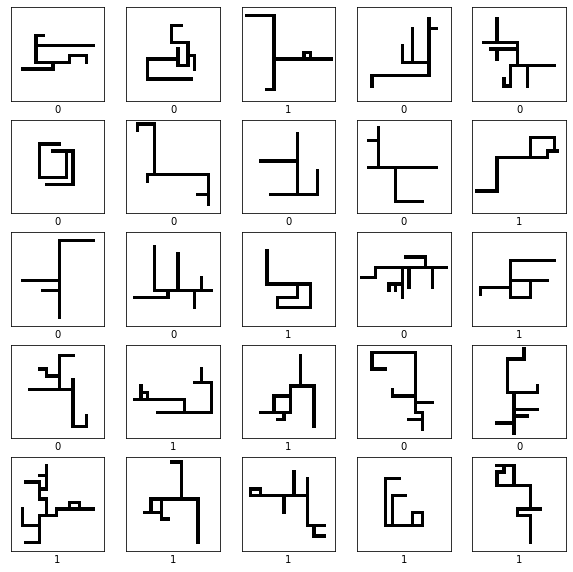
\includegraphics[width=1.0\textwidth]{../image/img25.png} %插入图片,[]中设置图片大小,{}中是图片文件名
    \caption{Cycle Dataset} %最终文档中希望显示的图片标题
    \label{Fig.img25} %用于文内引用的标签
\end{figure}

\section{Method}

\subsection{Deterministic algorithm of cycle detection problem}

\subsubsection{General Structure}

Let us consider how we can solve the cycle-recognization problem with a deterministic algorithm (BFS).
We call a pixel with value $1$ a positive pixel and a pixel with value $0$ a negative pixel.  
We only need to randomly choose a positive pixel, and know the distance of every pixel to the chosen pixel. 
Here, the distance means the minimum number of steps to reach the chosen positive pixel by only stepping to the neighbor \textbf{positive} pixels, 
and the neighbor pixels are up, down, left, and right pixels, so at most four pixels.
If we get the distance of every pixel, noticing that every cycle is an even cycle in this problem, 
so we only need to detect whether there are patterns a pixel with distance $d$ has at least two neighbor pixels with distance $d-1$.

So we have three parts in this algorithm:

\subsubsection{Initializer}

Given the image, we will initialize the distance of every pixel to the chosen positive pixel by 
choosing a random positive pixel and setting its distance to $0$, and setting all other pixels to $+\infty$.

\subsubsection{Solver}

Input the distance data output by the initializer, 
and do distance propagation operation repeatedly until all distance remains unchanged. 

A distance propagation operation is to set the new distance of every pixel to the minimum of the old distance and the distance adding one of its neighbor positive pixels.

That is: 

First, we let $d \mathrel{+}= inputs \cdot \infty$. That is using inputs as a mask. Here inputs is the original image that has $28*28\;$ $0$ or $1$. 

Then, we let $d = padding(d, 1, 1, +\infty)$. That is to padding a $+\infty$ with width $1$.

Finally, for all possible (i,j): 
$$d_{new}[i,j] = \min(d[i,j], d[i+1, j] + 1, d[i-1, j] + 1, d[i, j+1] + 1, d[i, j-1] + 1)$$

Notice that we use the same raw inputs in each solver. We call this method as using global inputs.


\subsubsection{Extractor}

An extractor is to extract the distance data from the solver output. 

We get the distance of every pixel from the output of the solver, 
and the extractor detects whether there are patterns a pixel with distance $d$ has at least two neighbor pixels with distance $d-1$.
If there are, output $1$, showing that the image contains a cycle, else output $0$.

That is:

\begin{align*}
    v& = d[i,j]                                       \\
    l& = [d[i,j-1], d[i-1,j], d[i+1,j], d[i,j+1]] - v \\
    d&[i,j] = sum(l == -1) >= 2 \\
    o&utputs = Any(d)
\end{align*}

If any $d[i,j]$ outputs $1$, then there is a cycle, and Extracor return $1$, else return $0$.

\begin{figure}[H] %H为当前位置,!htb为忽略美学标准,htbp为浮动图形
\centering %图片居中
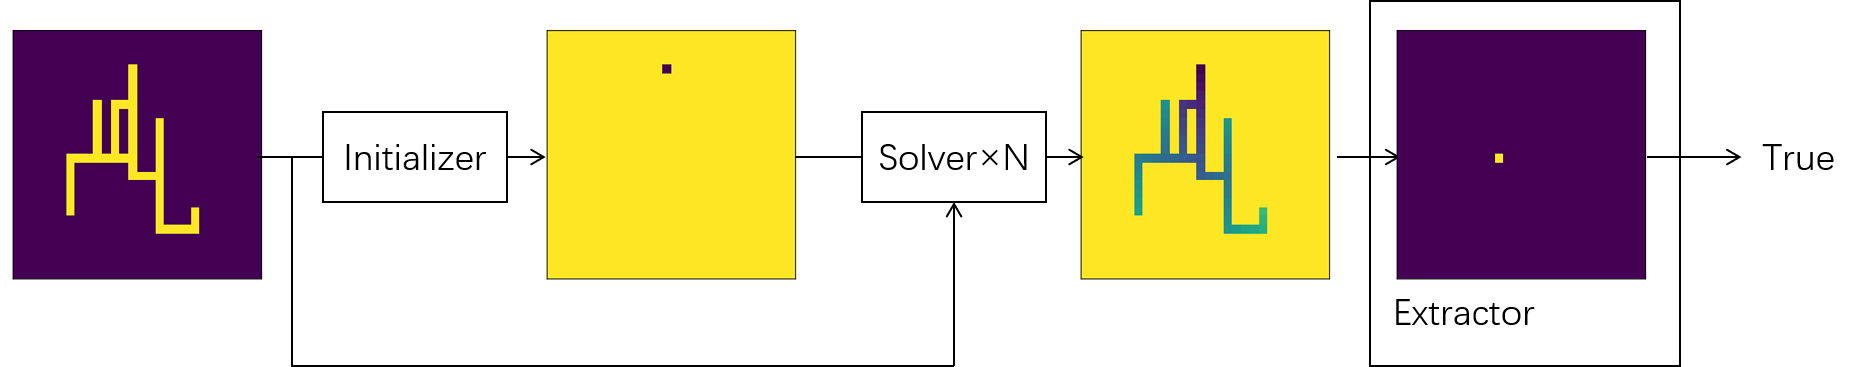
\includegraphics[width=1.0\textwidth]{../image/flow.png} %插入图片,[]中设置图片大小,{}中是图片文件名
\caption{Data Flow of Deterministic Algorithm in Cycle Recognization} %最终文档中希望显示的图片标题
\label{Fig.Flow} %用于文内引用的标签
\end{figure}

\subsection{GenCNN on Cycle Dataset}


\subsubsection{General Structure}

This model, GenCNN, is a neural network implementation of the above deterministic algorithm.

The model contains three parts: an initializer, a solver, and an extractor.

The initializer is used to initialize the initial state of a problem. 
The solver is used to solve the problem.
The extractor is used to extract the result of the problem from the solver.

It is very similar to the deterministic algorithm, but we use pytorch's neural network and functional API to implement it.

\begin{figure}[H]
\centering
\begin{minipage}{.5\textwidth}
    \centering
    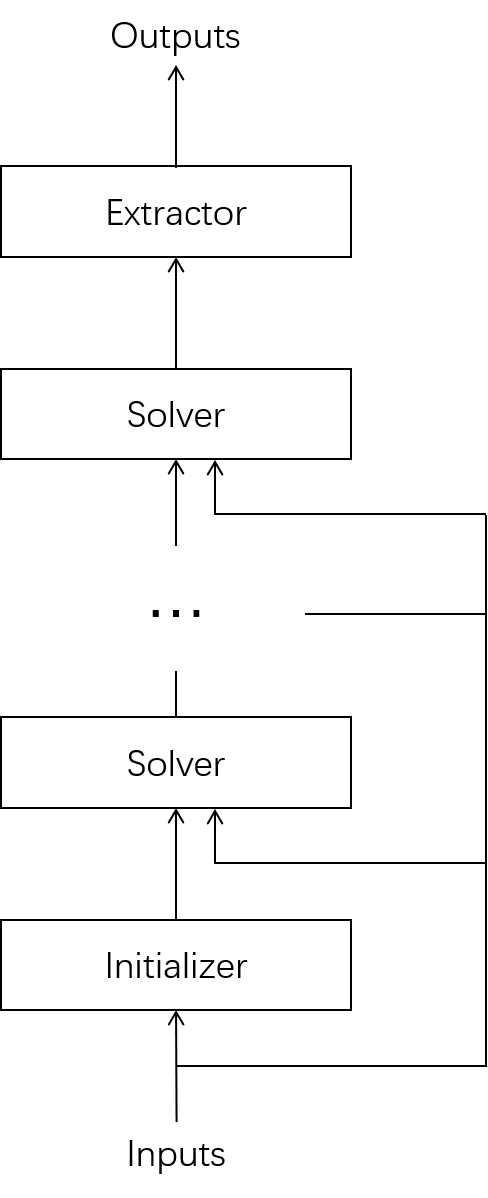
\includegraphics[width=.6\linewidth]{../image/model.png}
    \caption{GenCNN Architecture}
    \label{fig:fig1}
\end{minipage}%
\begin{minipage}{.5\textwidth}
    \centering
    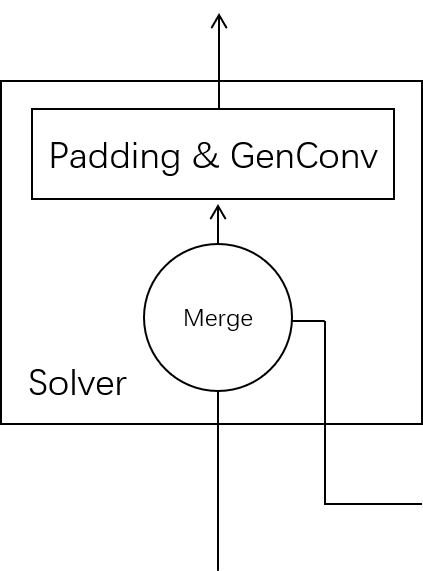
\includegraphics[width=.6\linewidth]{../image/solver.png}
    \caption{Solver Architecture}
    \label{fig:fig2}
\end{minipage}
\end{figure}

\subsubsection{Initializer}

The initializer is to randomly choose a positive pixel. That is not that easy to implement by pure neural network, so we use hard logic here.

\subsubsection{Solver}

As for the solver, we notice that the solver works like ConvNet, so we can call the solver a GenConv (Generalized Convolution Network).

ConvNet is $x_{new} = \sigma(\Sigma w_ix_i + b)$. $x_i$ is a neighborhood point of $x$, while GenConv is $x_{new} = f(X)$.

We call $f$ GenKernel, and this is how the name of GenCNN comes.

When handling the cycle dataset, since we want to have a finite representation of the infinite $f$, 
we use a MultiLayerPerceptron (MLP) as the GenKernel.

The inputs to the GenKernel is 5-D tensor, the outputs to the GenKernel is a 1-D tensor.

To represent the formula

$$d_{new}[i,j] = \min(d[i,j], d[i+1, j] + 1, d[i-1, j] + 1, d[i, j+1] + 1, d[i, j-1] + 1)$$

We use ReLU as the activation function of MLP.

Notice that $\min(a, b) = a - relu(a - b)$, and we can solve this problem.

The conclusion is that we can use a MLP whose width is 5-3-2-1 and choose ReLU as the activation function to build the solver part.

\subsubsection{Extractor}

The method we used to build the extractor part is similar to the solver part.

We still use MLP and ReLU to build the extractor part.

\begin{align*}
    v& = d[i,j]                                       \\
    l& = [d[i,j-1], d[i-1,j], d[i+1,j], d[i,j+1]] - v \\
    d&[i,j] = sum(l == -1) >= 2 \\
    outputs = Any(d)
\end{align*}

The only difficult part is the last two steps.

Notice that $1_{a<b} = min(relu(b-a)*10000,1)$, so we can compare two value using relu easily.

The third step (extract kernel step) can be rewrite as $d[i,j] = sum(-1.5\leq l \leq -0.5) >= 2 $, and we are done.

The last step (or step) $outputs = Any(d)$ can be represented as $outputs = \sum(relu(d)) > 0.001$, and we are done.

\section{Analysis}


\subsection{In the viewpoint of Graph Convolution Network}

Graph Convolution Network (GCN) is a generalization of Convolution Network (CNN).

GenCNN can also be used in a graph, and we can understand it as a variant of GCN \cite{kipf2016semi} (Graph Convolutional Network).

It overcomes the depth restriction of GCN being too smooth when the depth is too deep \cite{zhang2019graph}, since
the usage of global inputs and different GenKernel changed the fixed point.



\subsection{In the viewpoint of Cellular Automata}

GenKernel perfectly simulated evolutionary functions in cellular automata(CA), 
because in every evolution step of CA, the state of every cell is a function of the state of its neighborhood.

GenKernel $f$ defined all the possible function.

So everything CA can done can be done by GenCNN theoretically.

\subsection{More Generalized Model}

\subsubsection{Preparer}

A more general GenCNN model has a preparer. 

Notice that if in your dataset, each pixel does not contains much logical information but the visual type of perceptual information,
you should first add a preparer, which is a CNN-like part to extract the logic information before the logic information goes to the GenCNN part. 
In the model we used in handling the cycle dataset, we do not use preparer, 
because every pixel has logical information to determine whether there is a cycle in the image.

Actually, when handling cycle dataset, the solvers try to solve the distance of every pixel to a certain pixel. 
This is exactly finding the fixed point of the distance regarding to the relaxation operation.

\begin{figure}[H] %H为当前位置,!htb为忽略美学标准,htbp为浮动图形
    \centering %图片居中
    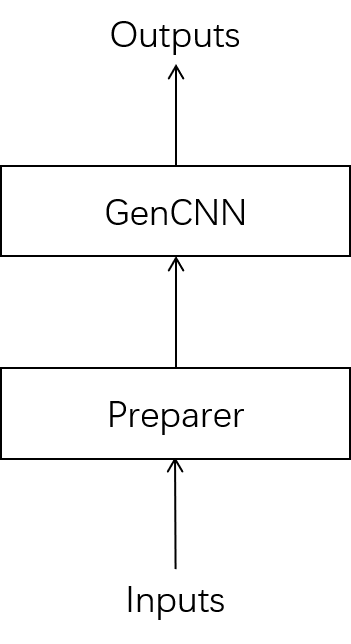
\includegraphics[width=0.3\textwidth]{../image/gen.png} %插入图片,[]中设置图片大小,{}中是图片文件名
    \caption{General GenCNN Architecture} %最终文档中希望显示的图片标题
    \label{Fig.GenCNN} %用于文内引用的标签
\end{figure}


\subsubsection{MultiChannel}

A more general GenCNN model has multi-channels just like traditional CNN, which is equivalent to holding a vector or tensor instead of a single value in $d[i,j]$. 
In this case, the GenKernel will be more complex, mapping from many tensors to a single tensor. 

Using this method GenCNN can solve more problems. For example, $d[i,j]$ can record the pixels that has certain relation with the pixel $i,j$, 
like, belongs to the same connected component, though there will be more time cost.

The total time cost is $depth\times image\_size^2 \times kernel\_cost$.

\subsubsection{Different Initializer, Solver and Extractor}

The structure of the initializer, the solver, and the extractor can be changed. 

For example, every solver can either use the same or different GenKernel.

Extractor can use MLP to extract the information like AlexNet \cite{krizhevsky2012imagenet}.

There are still much to be done.

\section{Experiments}

We first build a cycle dataset.

Then we do the following experiments on this dataset:

\begin{itemize}
    \item Build a deterministic algorithm to find the cycle.
    \item Build a GenCNN model to find the cycle.
    \item Use autogluon, an automl tool, to find the cycle.
\end{itemize}



Because the training time is too long (because of the cost of MLP), we did not train the GenCNN model.

The first and second methods can achieve 100\% accuracy, while the third method cannot.

Though ResNet-50 uses the mechanism of residuals, which is equivalent to global inputs, thus also achieving good results, 
it still misclassified some images.

\begin{figure}[H]
    \centering
    \begin{minipage}{.5\textwidth}
        \centering
        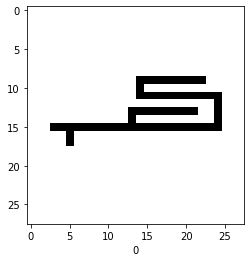
\includegraphics[width=.6\linewidth]{../image/miss1.png}
        \label{fig:miss1}
    \end{minipage}%
    \begin{minipage}{.5\textwidth}
        \centering
        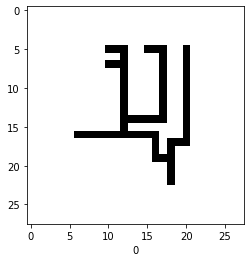
\includegraphics[width=.6\linewidth]{../image/miss2.png}
        \label{fig:miss2}
    \end{minipage}
    \caption{Two misclassified images by ResNet-50}
\end{figure}

\section{Future Work}

\subsection{Dataset}

The cycle dataset is too easy. We need more difficult deterministic datasets.

The question is whether we can generate more questions and answers with good distribution, 
but hard to solve by the classical algorithm. We know this kind of problems exist, 
that is integer decomposition, but it is not friendly to the neural network.

In short, we need more questions and data generation methods.

\subsection{GenKernel}

Further experiments can replace the MLP with a simpler GenKernel and increase its speed.

\subsection{Loop Logic}

We also noticed that current neural network have an incapacity of loop logic. 
That makes the GenCNN, RNN, and a lot of other models to be deep to simulate static loop unfolding, 
and that is not a good thing.
Also, no current neural network can handle dynamic loop. 
This will lead to an unreasonable increase in time comparing to deterministic algorithm.

For example, what the initializer of GenCNN handling cycle dataset do now is to randomly choose a positive pixel.
Let $n$ be the number of pixels.
This is easy to do in $O(n)$ in the deterministic algorithm. We can choose the first $1$ we meet, and not choose other pixels.
But in neural network, we need to determine whether to choose a pixel by $O(n)$, and the total time would be $O(n^2)$.
That is not a good time complexity.

Our ultimate goal is to be able to implement all algorithmic logic with neural networks.

\section{Conclusions}


In this paper, we hope to draw attention to the general incompetence of neural networks for strong logic problems, 
and to arouse interest in solving it with cycle dataset. 
Our ultimate goal is to be able to implement all algorithmic logic with neural networks.

The new model GenCNN proposed in this paper is of value as an attempt to solve the problem, 
while changing the convolution and activation functions to arbitrary functions, 
extending the traditional form of convolution and greatly enhancing the capabilities of CNN, 
adding global inputs to solve the oversmooth problem of GCN.


\section*{Acknowledgements}

Thanks my teacher Weinan Zhang for teaching me.

Thanks Jiaming Tang for the idea support.

Thanks my friends who give me courage to try new methods and ideas.

\medskip

\bibliographystyle{plain}

\bibliography{ref}


% \appendix


% \section{Appendix}


% Optionally include extra information (complete proofs, additional experiments and plots) in the appendix.
% This section will often be part of the supplemental material.


\end{document}